\section{Sistema Decimal a Sistema Binario}

\subsection{Descripción del problema}
Se solicita que los números decimales se conviertan a números binarios como en positivos y negativos 
\begin {figure}[h!]
\centerline{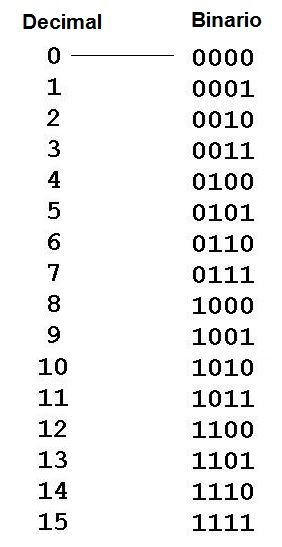
\includegraphics[width = 4cm]{imagen/numeros-binarios.jpg}}
\caption{Binario a decimal.}
\label{fig}
\end {figure}

\subsection{Definición de solución}
Primero se identifican si el número decimal es un entero positivo o negativo, también se le implementara el complemento a dos la cual se ocupa cuando un numero decimal es negativo.
\subsection{Diseño de Solución}
Se solicita un numero decimal, ya sea positivo o negativo, este  sera convertido a numero binario en el cual, se dividirá entre 2 y el resultado también sera divido en 2 hasta que ya no se pueda dividir mas; si el numero decimal es negativo, al convertirlo en binario se hará el mismo procedimiento pero se le impondrá el complemento a dos, en donde se invertirán los bits y se le sumara 1 dándonos hacia el numero binario negativo 
\subsection{Desarrollo de Solución}
\begin{javaCode}
    Scanner scanner = new Scanner(System.in);

        System.out.print("Ingresa un número decimal: ");
        int numeroDecimal = scanner.nextInt();

        String numeroBinario = convertirABinario(numeroDecimal);

        System.out.println("El número binario equivalente es: " + numeroBinario);
    }

    private static String convertirABinario(int numeroDecimal) {
        StringBuilder binario = new StringBuilder();

        if (numeroDecimal == 0) {
            return "0";
        }

        boolean esNegativo = false;
        if (numeroDecimal < 0) {
            esNegativo = true;
            numeroDecimal = -numeroDecimal;
        }

        // Convertir el número decimal a binario
        while (numeroDecimal > 0) {
            int residuo = numeroDecimal % 2;
            binario.insert(0, residuo);
            numeroDecimal /= 2;
        }

        // Calcular el complemento a dos si el número es negativo
        if (esNegativo) {
            // Invertir los bits
            for (int i = 0; i < binario.length(); i++) {
                char bit = binario.charAt(i);
                binario.setCharAt(i, (bit == '0') ? '1' : '0');
            }
            
            // Sumar 1 al complemento invertido
            int carry = 1;
            for (int i = binario.length() - 1; i >= 0; i--) {
                int bit = (binario.charAt(i) - '0') + carry;
                binario.setCharAt(i, (char) (bit % 2 + '0'));
                carry = bit / 2;
            }
        }

        return binario.toString();
    }
}
\end{javaCode}

\subsection{Depuración y pruebas}
\begin{tabular}{|c|c|c|c|}
  \hline
  NumCorrida &Decimal & Binario & C2  \\
  \hline
  1 & 5 & 101 & 1011 \\
  \hline
  2 & 20 & 10100 &  11101100 \\
  \hline
  3 & 60 & 111100 & 11000100\\
  \hline
  
\end{tabular}
